\documentclass{beamer}

\usepackage[beamer]{shortcut}
\usepackage{bibentry}

\graphicspath{{./images/}}
\usepackage[square]{natbib}



\newcommand{\rightcite}[1]{\keypoint{\small[{\color{linkcolor} #1}]}}
\newcommand{\bottomlink}[1]{\vspace{0pt plus 1 filll}\rightcite{#1}}

\newcommand{\techterm}[1]{
	\column{\widthof{\bf #1g}}
    \centering
    \begin{beamercolorbox}[rounded=true, shadow=true]{title}%
        {\centering\bf #1\hskip-1ex\phantom{g}\\}
    \end{beamercolorbox}%
}

\newcommand{\highlightbox}[1]{
    \begin{beamercolorbox}[rounded=true,
                           shadow=true]{title}
        #1
    \end{beamercolorbox}}


\def\keypoint#1{\hspace{0pt plus 1 filll}\textcolor{gray}{#1}}
\def\mycite#1{\keypoint{\small\citep{#1}}}
\def\tT{\widetilde{T}}
\def\myitem{\hskip1ex{\color{linkcolor} $\blacktriangleright$}\hskip.3em}

\institute{\\ INRIA Saclay - MIND Team}
\author{Thomas Moreau}
\title{
	Unsupervised signal processing with ML tools
}

\setbeamertemplate{title page}[frame]
\def\extraLogo{}

\begin{document}

\begin{frame}
	\titlepage
    \nobibliography{library.bib}
\end{frame}


\frame{
    \frametitle{Who am I?}

    \begin{itemize}\itemsep2em
        \item CR Inria
        \item Working on unsupervised representations for signals
        \item Recent focus on bi-level optimization and point processes
        \item Application to Neuroimaging
        \item Open source software contributor
    \end{itemize}

    {\centering\hfill
    \includegraphics[height=5em]{logo_benchopt}\hfill
    \includegraphics[height=5em]{logo_joblib}\hfill
    \includegraphics[height=5em]{logo_loky}\hfill\\
    }

}


\frame{
    \frametitle{}

    \begin{columns}[c]
        \column{.6\columnwidth}
    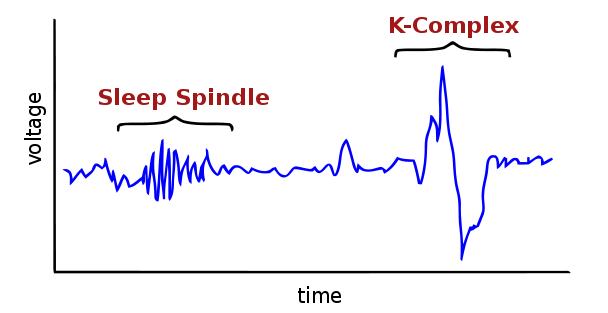
\includegraphics[width=\textwidth, trim={6em 6em 0 0}, clip]{sleep_spinddle}
        \column{.35\columnwidth}
            \highlightbox{
                \centering \Large
                Neural signals exhibit
                diverse and complex
                morphologies
            }
    \end{columns}
    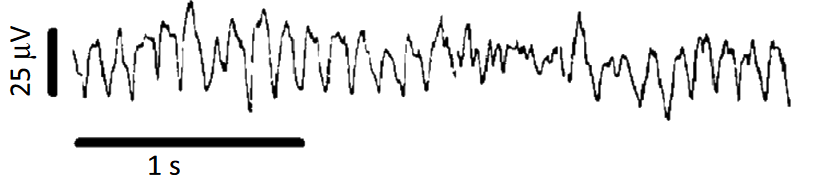
\includegraphics[width=\textwidth]{mu_rythm}\\[-1.5em]
    \rightcite{Cole \& Voytek 2017}
    \vskip-7em
        \begin{columns}[c]
        \column{.75\columnwidth}
        \visible<2->{\highlightbox{\vskip.1em
        \Large Waveform shape can be related to diseases\\
        \eg{} Parkinson \rightcite{Jackson et al. 2019}}\\[.3em]}
        \end{columns}
    \vskip3em
    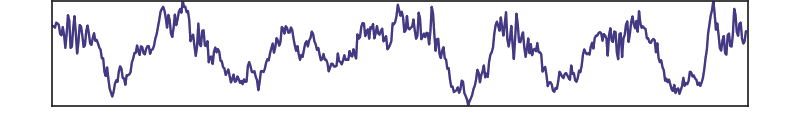
\includegraphics[width=\textwidth]{cfc}\\[-.8em]
    \rightcite{\footnotesize Dupré la Tour et al. 2017}
}


\frame[t]{
	\frametitle{Convolutional Dictionary Learning}

    \textbf{Key idea}: decouple the localization of the
                        patterns and their shape
    \vskip.5em%
    \centering
    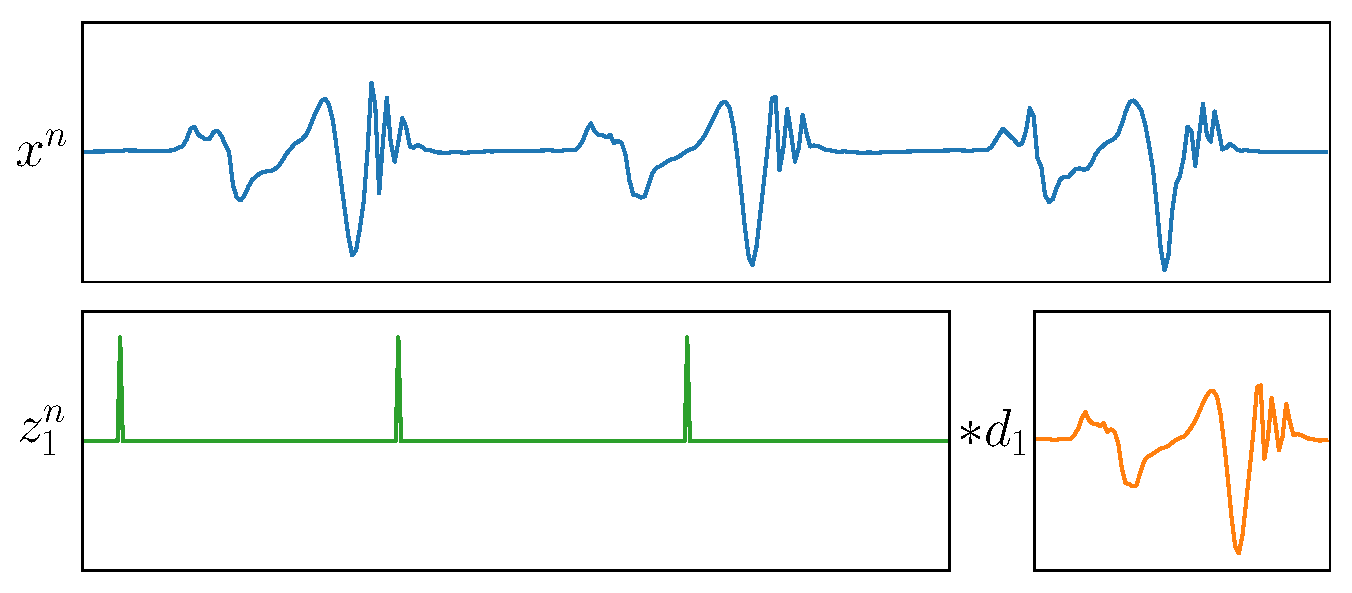
\includegraphics[width=\textwidth]{intro_csc_5}
    \vskip0em%
    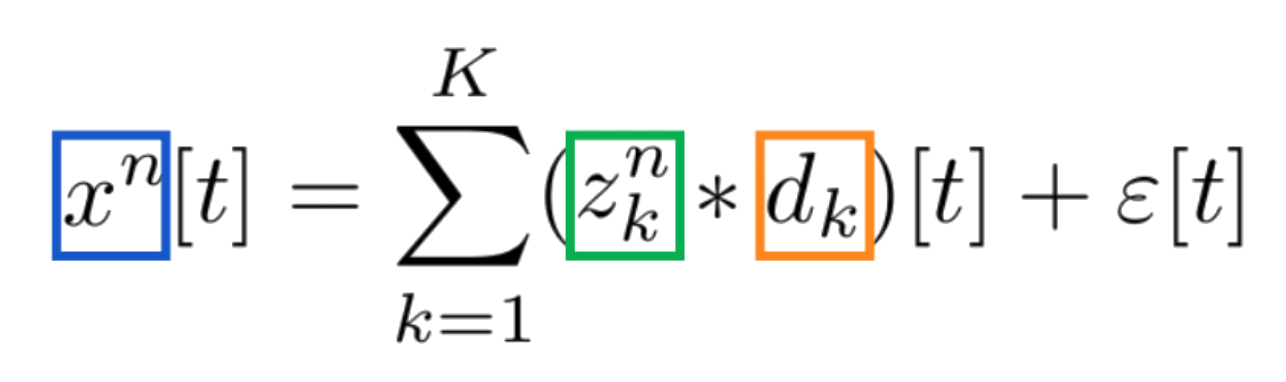
\includegraphics[width=.6\textwidth]{csc_explain_eq_color}%
}

\frame{
    \frametitle{Bi-level optimization}

    {\bf Bi-level problem:} Optimization problem with two levels\\[1em]
    \begin{align*}
        \min_\lambda ~& {\color{darkblue} h(\lambda)} = {\color{darkred}F(\lambda, \theta^*(\lambda))} \\[.5em]
            & s.t.\quad \theta^*(\lambda) = \argmin_\theta {\color{lightgreen}G(\lambda, \theta)}
    \end{align*}
    \begin{tikzpicture}[overlay]
        \draw[<-, thick, shorten >=8, darkblue] (4.1, 1.7) -- +(-1.5, -1.3) node[darkblue] {\emph{Value function}};
        \draw[<-, thick, shorten >=35,darkred] (7.3, 1.9) -- +(3, -.2) node {\emph{\color{darkred}Outer function}};
        \draw[<-, thick, shorten >=8, lightgreen] (8, .5) -- +(0, -.8) node {\emph{\color{lightgreen} Inner function/Problem}};
    \end{tikzpicture}

    \vskip3em
    {\bf Challenge:} How to solve it without solving the inner problem many times?
}


\begin{frame}{MNE sample data}
    A selection of temporal waveforms of the atoms learned on the MNE sample dataset.\\[1em]
    \centering
    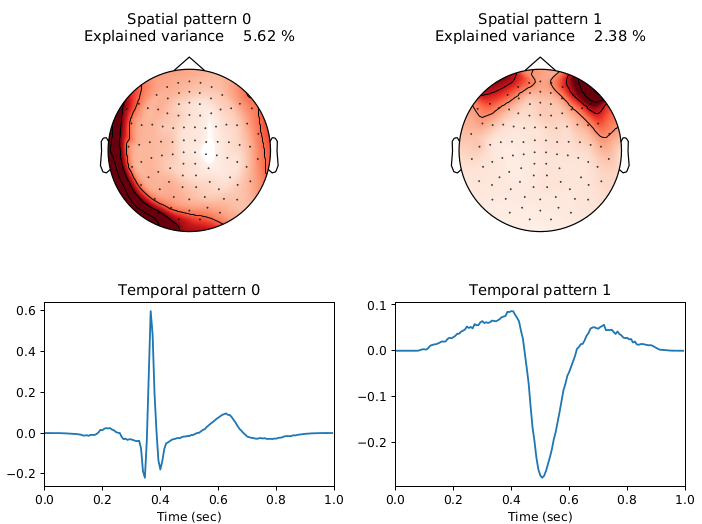
\includegraphics[height=0.7\textheight]{artifacts}
\end{frame}


\frame[t]{
    \frametitle{Learned atoms -- Evoked response}

    \centering
    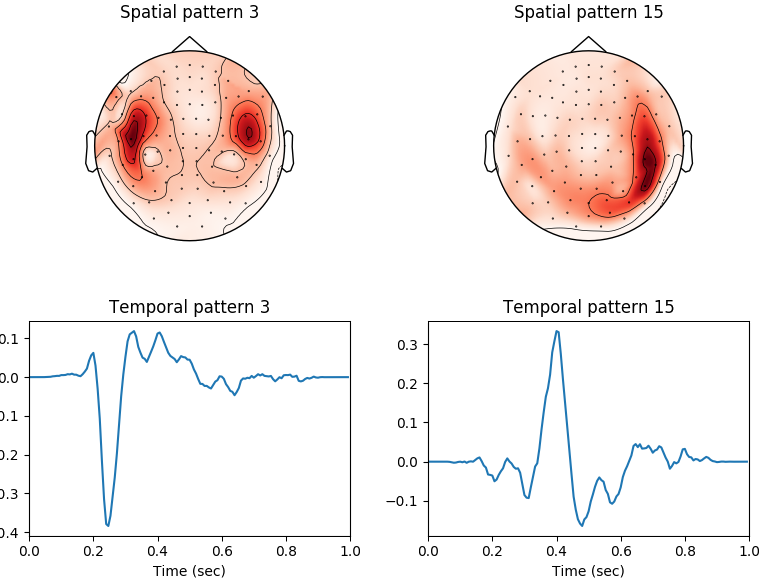
\includegraphics[width=.9\columnwidth]{evoked}
}



\frame{
    \frametitle{Statistical modeling: Stimuli Induced Patterns}

    \myitem{} Manual pattern identification\\[.5em]
    \myitem{} No quantification of how stimuli influence patterns activation.\\[1em]

    \centering
    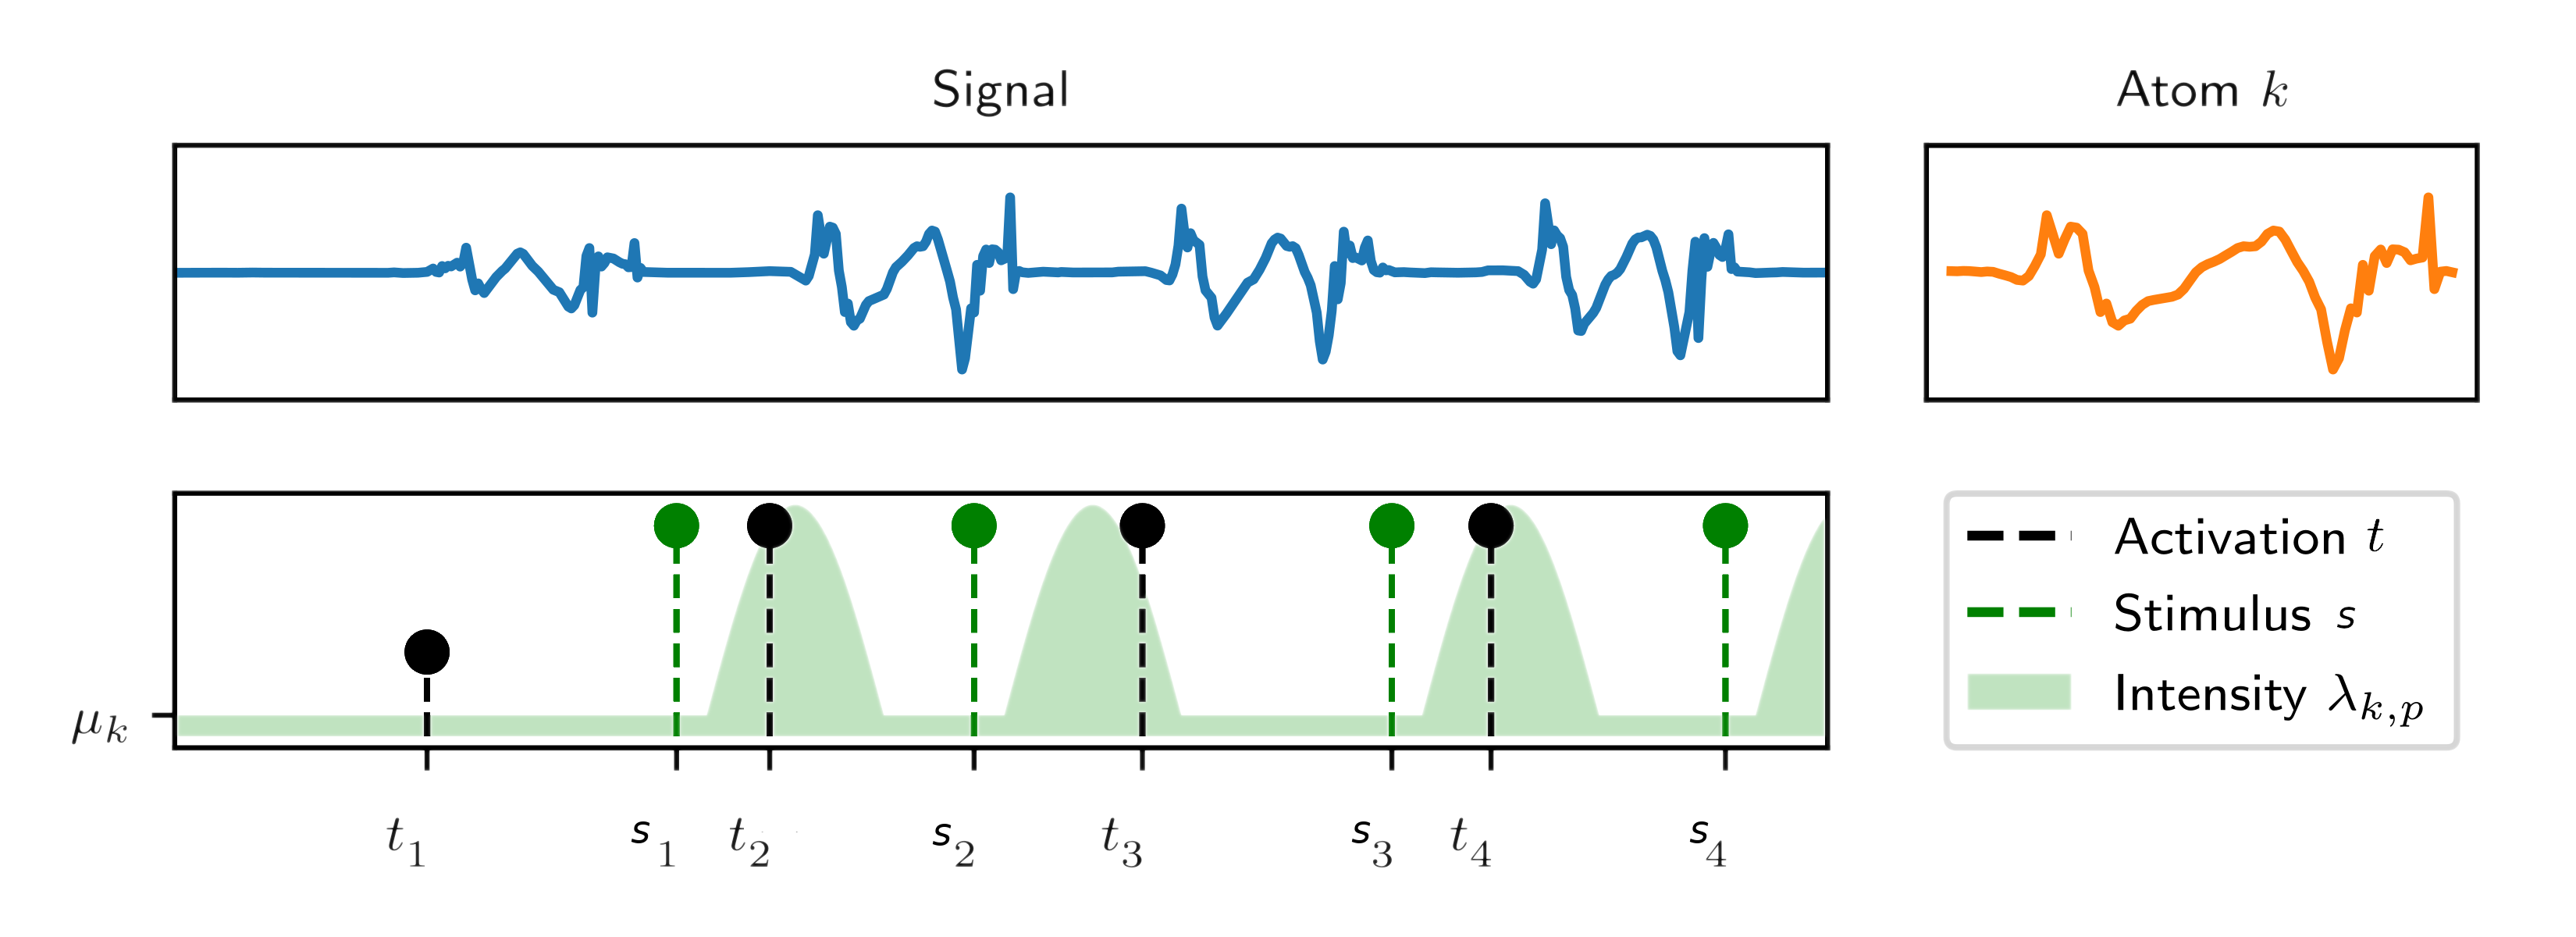
\includegraphics[width=\textwidth]{csc_and_pp.png}\\[1em]


    Activations and stimuli can be seen as \emph{Point Processes}.\\
    \rightcite{Allain2022}
}

{\usebackgroundtemplate{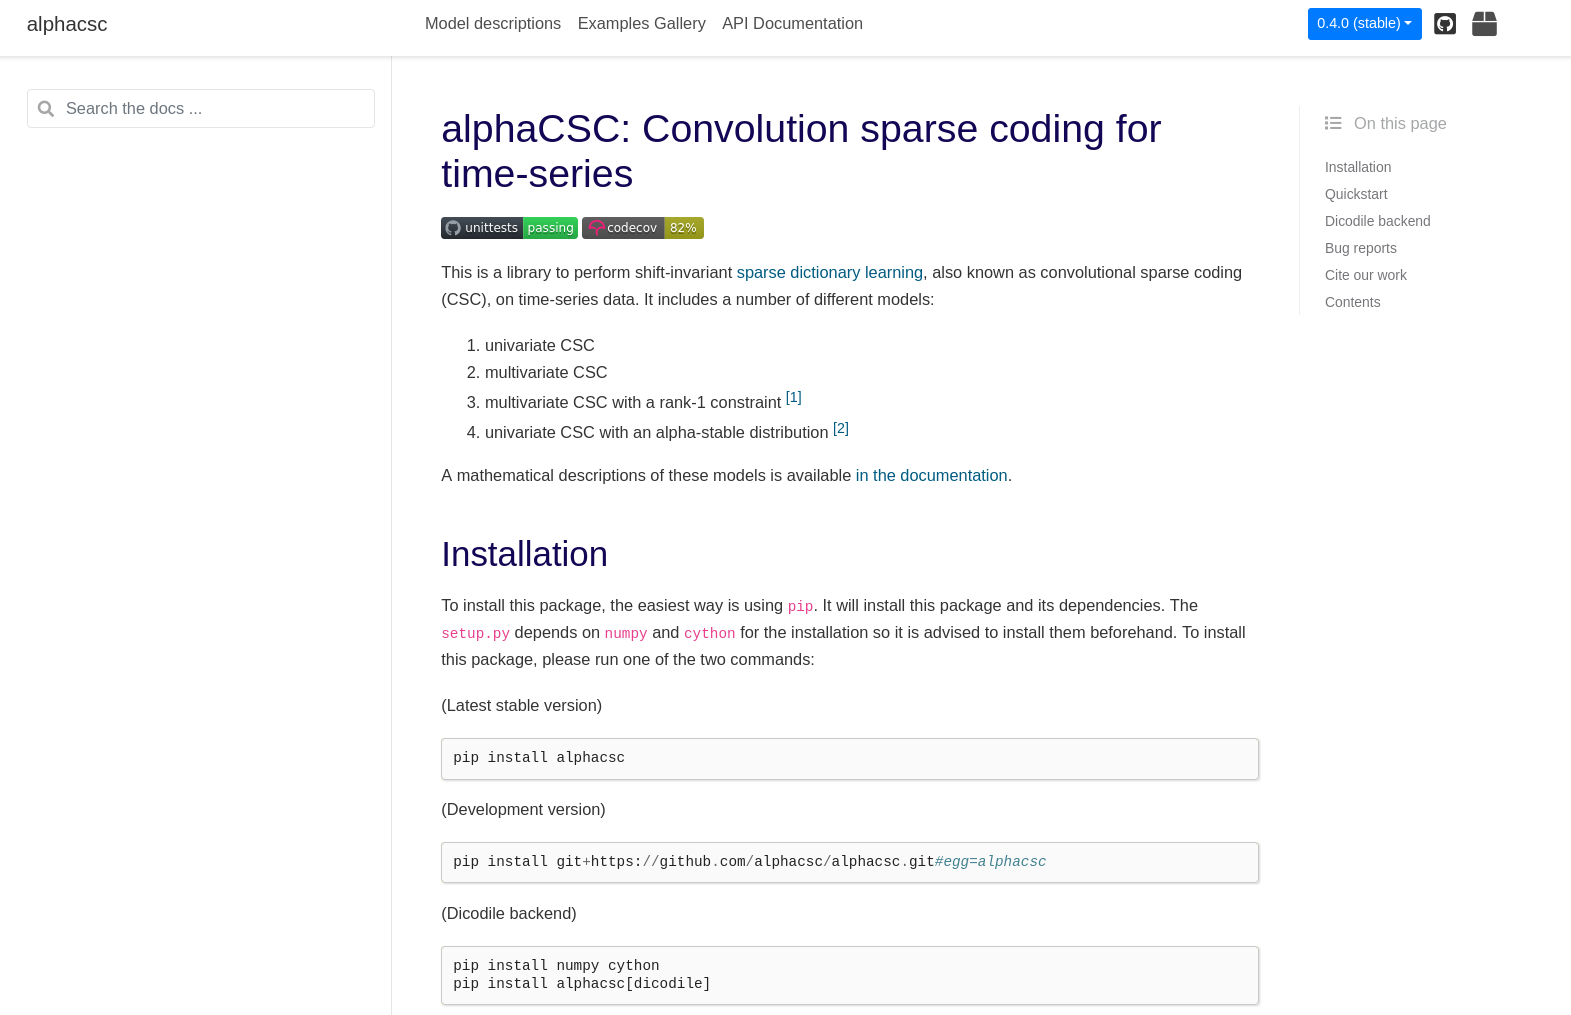
\includegraphics[width=\paperwidth]{alphacsc_04}}%
\frame{
    \begin{columns}
        \column{.5\textwidth}
        \column{.4\textwidth}
        \highlightbox{Python code online:\\
                        https://alphacsc.github.io\\[1em]
                        \texttt{pip install alphacsc}}
        \vskip2em
            \highlightbox{Examples reproduce figures from this talk!}

    \end{columns}
}}


\frame{
    \frametitle{Benchopt}
    \centering
    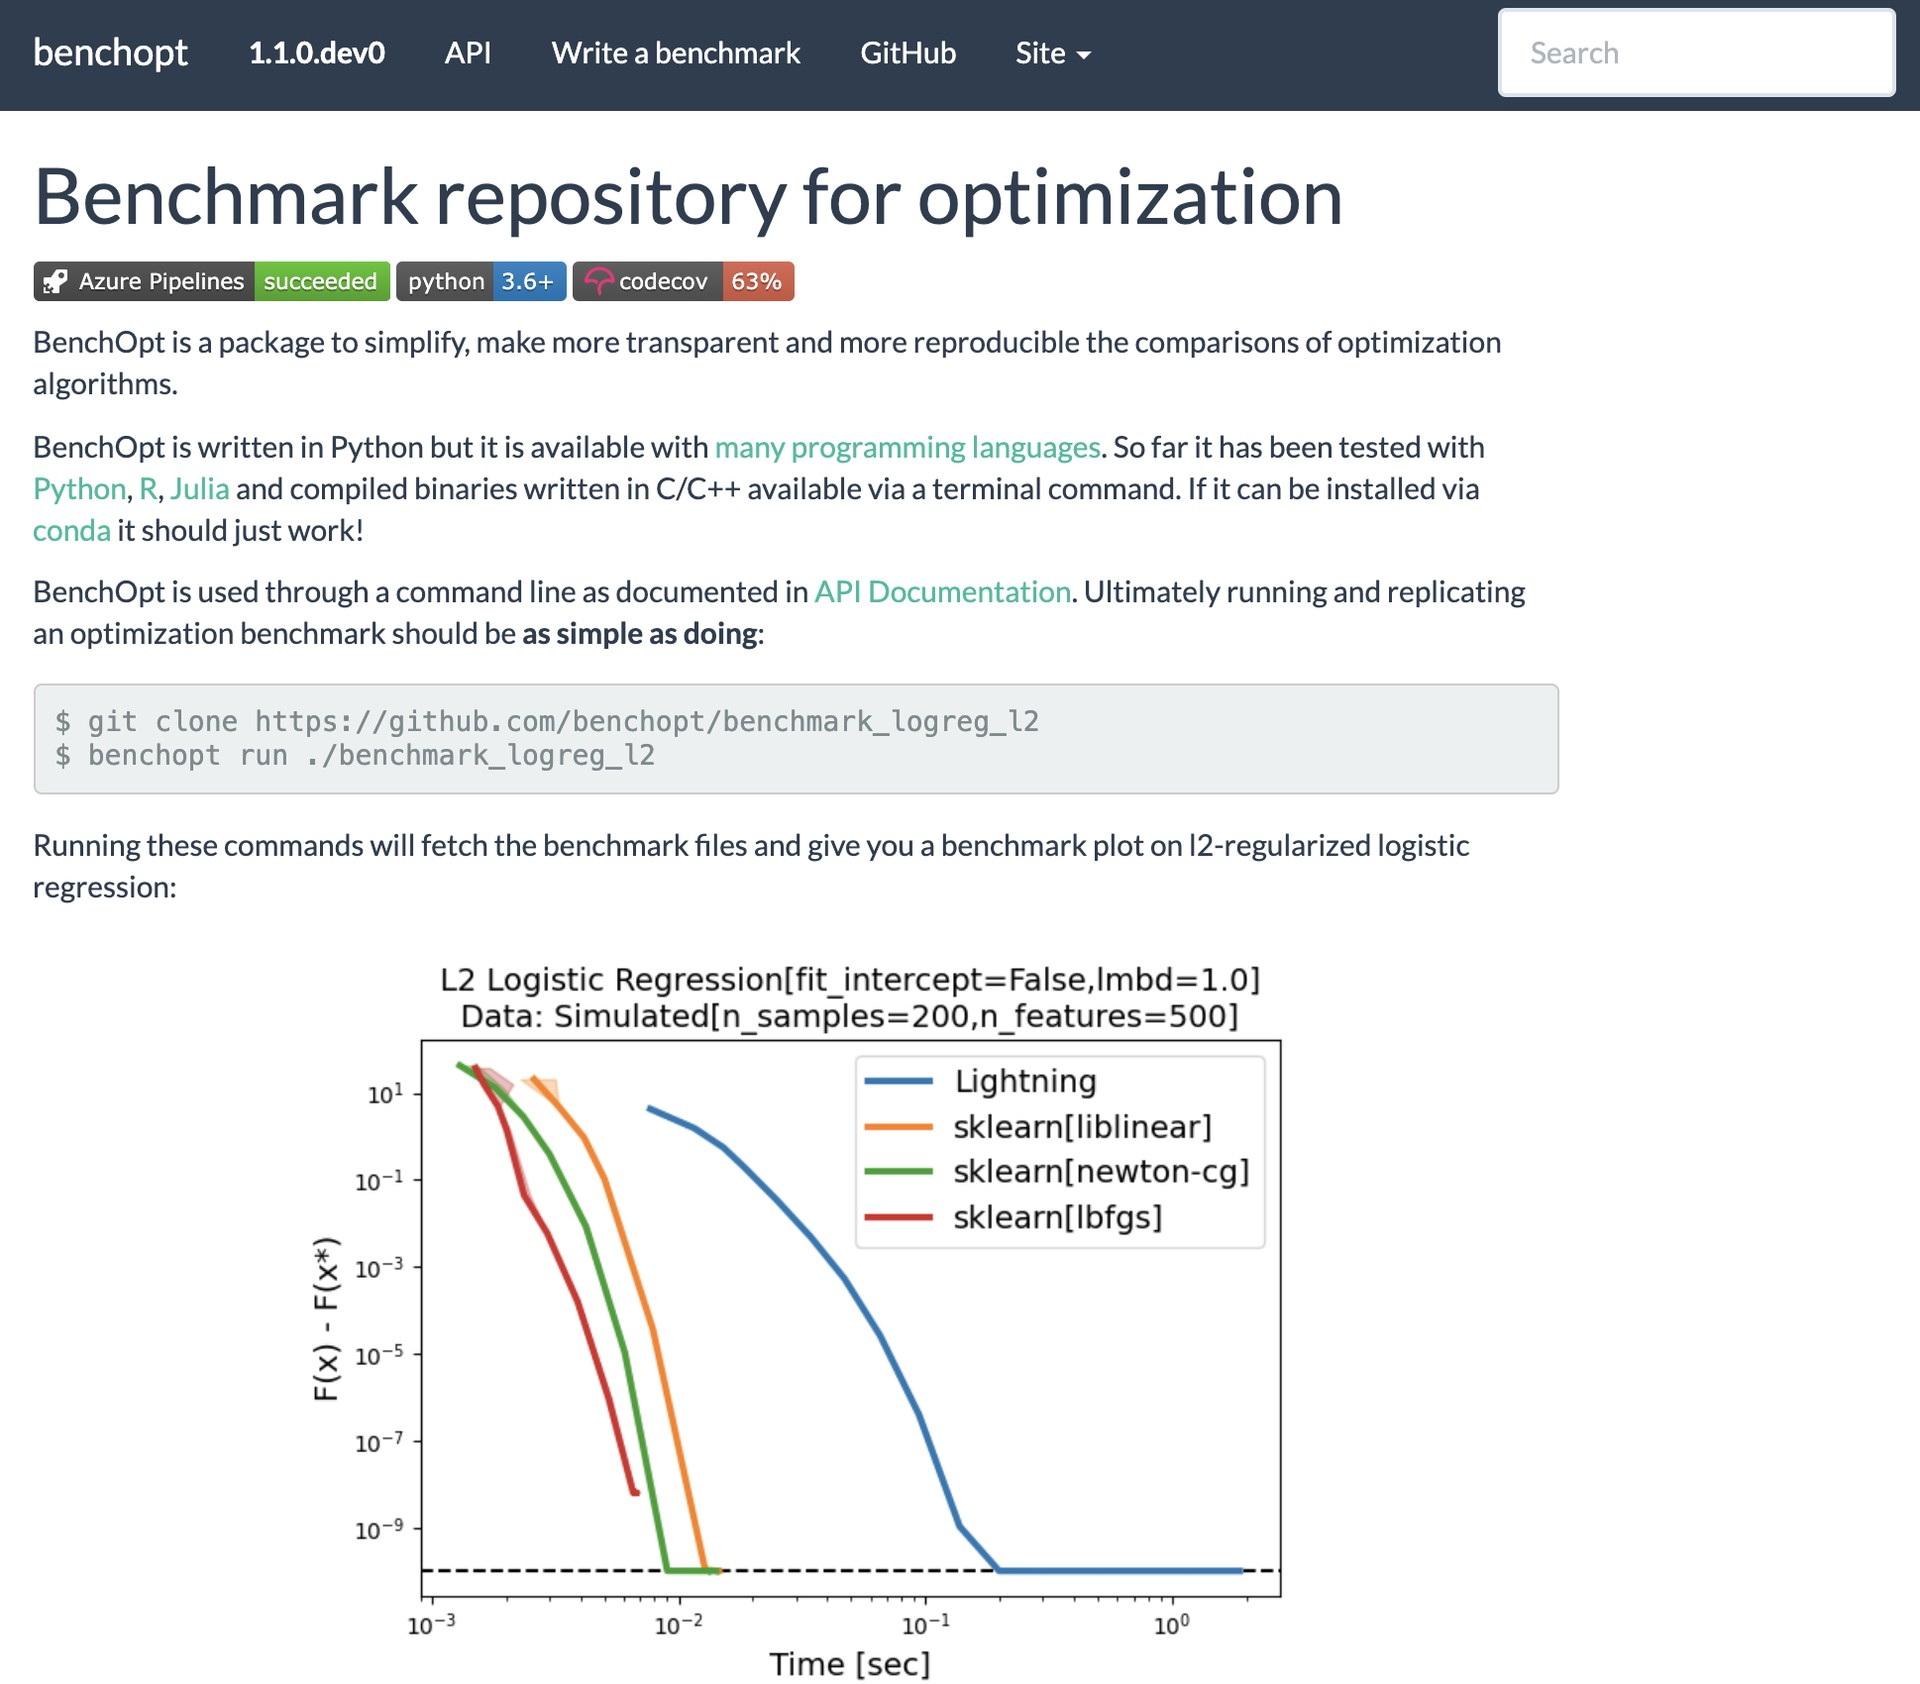
\includegraphics[width=.9\textwidth]{benchopt}\\
}


\frame{
    \vskip2em
    {\centering
        \usebeamercolor[fg]{title}
        \usebeamerfont{title}
        \Huge \bf Thanks for your attention!\\[2em]}

    Code available on my github: \href{https://github.com/tommoral/}{\texttt{@tommoral}}\\[2em]

    Slides are on my web page:\\[1em]
    \hskip5em\includegraphics[height=.8em]{website} tommoral.github.io
    \hskip4em 
\includegraphics[height=.8em]{twitter} @tomamoral

}



\end{document}
